% 
% Annual Cognitive Science Conference
% Sample LaTeX Paper -- Proceedings Format
% 

% Original : Ashwin Ram (ashwin@cc.gatech.edu)       04/01/1994
% Modified : Johanna Moore (jmoore@cs.pitt.edu)      03/17/1995
% Modified : David Noelle (noelle@ucsd.edu)          03/15/1996
% Modified : Pat Langley (langley@cs.stanford.edu)   01/26/1997
% Latex2e corrections by Ramin Charles Nakisa        01/28/1997 
% Modified : Tina Eliassi-Rad (eliassi@cs.wisc.edu)  01/31/1998
% Modified : Trisha Yannuzzi (trisha@ircs.upenn.edu) 12/28/1999 (in process)
% Modified : Mary Ellen Foster (M.E.Foster@ed.ac.uk) 12/11/2000
% Modified : Ken Forbus                              01/23/2004
% Modified : Eli M. Silk (esilk@pitt.edu)            05/24/2005
% Modified : Niels Taatgen (taatgen@cmu.edu)         10/24/2006
% Modified : David Noelle (dnoelle@ucmerced.edu)     11/19/2014

%% Change "letterpaper" in the following line to "a4paper" if you must.

\documentclass[10pt,letterpaper]{article}

\usepackage{cogsci}
\usepackage{pslatex}
\usepackage{apacite}
\usepackage{graphicx}
\usepackage{amssymb,amsfonts,amsmath}

\title{Let's talk (ironically) about the weather: A computational model of verbal irony}
 
\author{{\large \bf Justine T. Kao
(justinek@stanford.edu)} \\
  Department of Psychology, 450 Serra Mall \\
  Stanford, CA 94305 USA
  \AND {\large \bf Noah D. Goodman (ngoodman@stanford.edu)} \\
  Department of Psychology, 450 Serra Mall \\
  Stanford, CA 94305 USA}


\begin{document}

\maketitle


\begin{abstract}
Verbal irony plays an important role in how we communicate and express our opinions about the world. While there exist many interesting theories and empirical findings about how people use and understand verbal irony, there is to our knowledge no formal model of how people incorporate shared background knowledge and linguistic information to communicate ironically. Here we present two behavioral experiments that examine people's interpretations of utterances given different contexts in the weather domain. We then describe a computational model that reasons about background knowledge, affect, and the speaker's communicate goals to interpret ironic utterances and their rich affective subtexts. We show that by accounting for two types of affect goals---valence and arousal---our model produces interpretations that closely match humans'. Finally, we discuss the implications of our model on irony and its relationship to other types of nonliteral language understanding.


\textbf{Keywords:} 
irony; computational modeling; pragmatics; nonliteral language understanding
\end{abstract}


\section{Introduction}
For better or for worse, verbal irony---roughly defined as utterances whose apparent meanings are opposite in polarity to the speaker's intended meaning \cite{roberts1994people, colston2000contrast}---is a major figurative trope of our time. From popular sitcoms to political satire to \emph{\#sarcasm} on Twitter and casual conversations among friends, verbal irony plays an important role in how we communicate and express our opinions about the world. Given the prevalence of irony in natural language, many researchers in natural language processing aim to automatically detect sarcasm in large bodies of texts in order to recover the correct sentiment from an ostensibly positive or negative utterance (e.g. ``I was overjoyed to pay $\$30$ for an overcooked steak") \cite{davidov2010semi, filatova2012irony}. A critical insight that emerges from these approaches is that irony detection requires information far beyond surface linguistic cues, often calling upon a deep understanding of context and common knowledge between speaker and listener, which computers currently lack. Indeed, without sufficient contextual information, even human beings exhibit poor judgment of verbal irony \cite{gonzalez2011identifying, wallacehumans}. 

If irony is so difficult to understand, then why do we use it? Previous work has shown that verbal irony serves several important communicative goals, such as to highlight group membership \cite{gibbs2000irony}, heighten or soften criticism \cite{colston1997salting}, produce humorous effects \cite{roberts1994people}, express attitudes \cite{colston1998you, colston1997ve}, and elicit emotional reactions \cite{leggitt2000emotional}. These findings suggest that while ironic statements are false under their literal meanings, they are often highly informative with respect to social and affective dimensions of meaning. 

Linguists and psychologists have proposed different theories about how people recover the intended meaning of an ironic utterance. According to a classic Grecian analysis of irony using conversational maxims \cite{grice20134, wilson2006pragmatics}, a listener first needs to recognize that an ironic utterance blatantly violates the maxim of quality (to be truthful) in order to arrive at a conversational implicature that is contrary to the literal meaning of the utterance. However, Grice's account does not provide a satisfactory explanation for how the implicature is derived, or how the listener infers affective subtext from the utterance \cite{wilson2006pragmatics}. Since Grice's original proposal, there have been two competing theories of irony understanding. The echoic mention theory \cite{sperber1981irony, jorgensen1984test} proposes that ironic utterances are intended to remind the listener of a previous utterance that turned out to be false or irrelevant. The affective subtext of irony then arises from the contrast between what was said earlier and what is actually the case. On the other hand, pretense theory \cite{clark1984pretense} argues that when a speaker produces an ironic utterance, she is not genuinely making the utterance, but only pretending to be someone who would make such an utterance. Understanding an ironic statement then involves recognizing the pretense as well as the preposterousness of the person being enacted. (could make this whole part shorter) 

While these informal theories each offer interesting insights into certain aspects of irony, determining which particular theory is superior is beyond the scope of this paper. Instead, we are interested in identifying basic elements of irony that are consistent across different theoretical frameworks and providing a precise formal account of how these elements can be incorporated to produce ironic interpretations. We observe that across different approaches to verbal irony, researchers agree that common ground between speaker and listener is critical for successful interpretation \cite{williams1984does}. In addition, verbal irony almost always communicates the speaker's attitude about a certain topic (cite). While there are interesting theories and empirical findings about how people use and understand verbal irony, there is to our knowledge no formal model of how people incorporate shared background knowledge and linguistic information to communicate about the world and their attitudes using irony.

Here we present a computational model that takes into account common ground and affective dimensions of meaning to model how people understand irony. We propose an extension to the basic Rational Speech Act (RSA) model, which formalizes language understanding as recursive reasoning between speaker and listener \cite{frank2012predicting, goodman2013knowledge}. Previous work has shown that extending basic RSA models to incorporate the speaker's communicative goals produces interpretations of nonliteral language that closely match humans' \cite{kao2014nonliteral, kao2014formalizing}. In particular, a model that reasons about the speaker's affective goals is able to interpret hyperbolic utterances and infer the appropriate affective subtext \cite{kao2014nonliteral}. However, \cite{kao2014nonliteral} considered only one affective dimension, namely the presence or absence of negative feeling, ignoring the range of attitudes and emotions that speakers could express with nonliteral utterances. Given the particular importance of affective meanings in verbal irony, here we extend the model to consider a wider range of positive and negative emotions. 

In what follows, we will examine interpretations of potentially ironic utterances in an innocuous domain---the weather. We chose the weather as the victim of irony for several reasons. First, people are quite familiar with talking (and complaining) about the weather. Second, we can visually represent the weather to participants with minimal linguistic description to obtain measures of nonlinguistic contextual knowledge. Finally, we can vary the weather states to observe how the same utterance is interpreted differently given different contextual knowledge. We first  present two behavioral experiments that examine people's interpretations of utterances given different weather contexts. We then describe a computational model that reasons about background knowledge, affect, and the speaker's communicate goals to interpret ironic utterances and their rich affective subtexts. We show that by accounting for two types of affect goals, valence and arousal, our model produces interpretations that closely match humans'. Finally, we discuss the implications of our model on irony and its relationship to other types of nonliteral language understanding.

\section{Behavioral Experiments}
We conducted the following two experiments to elicit people's judgements of potentially ironic utterances and their relationship to context and background knowledge. In Experiment 1, we collected participants' ratings of various weather contexts as well as how a person (e.g. Ann) feels about the weather. The weather ratings measure knowledge of the current weather state. The affect ratings measure how people generally feel about different weather states, which captures people's intuitive theory of attitudes towards the weather. In Experiment 2, we collected people's ratings of Ann's judgment of and feelings towards the weather given what she says about it, for example, ``The weather is terrible!" when the weather depicted is clearly sunny and nice.

\subsection{Experiment 1: Prior elicitation}
\subsubsection{Materials and methods}
We selected nine images from Google Images that depict the weather. To cover a range of weather states, three of the images were of sunny weather, three of cloudy weather, and three of rainy or snowy weather. Each of these images represents a \emph{weather context}, or $w_i$. The images can be found here:

$49$ native English speakers with IP addresses in the United States were recruited on Amazon's Mechanical Turk. Each participant saw all nine images in random order. In each trial, participants were told that a person (e.g. Ann) looks out the window and sees the view depicted by the image. They then indicated how Ann would rate the weather using a labeled 5-point Likert scale, ranging from \emph{terrible}, \emph{bad}, \emph{neutral}, \emph{good}, to \emph{amazing}. Finally, participants used slider bars to rate how likely Ann is to feel each of the following seven emotions about the weather: \emph{excited}, \emph{happy}, \emph{content}, \emph{neutral}, \emph{sad}, \emph{disgusted}, and \emph{angry}. The order of the emotions were randomized for each participant but remained consistent across trials for the same participant. The end points of the slider bars were labeled as ``Impossible" and ``Absolutely certain." A link to the experiment is here:
  
\subsubsection{Results}
\begin{figure}[t]
\scalebox{0.4}{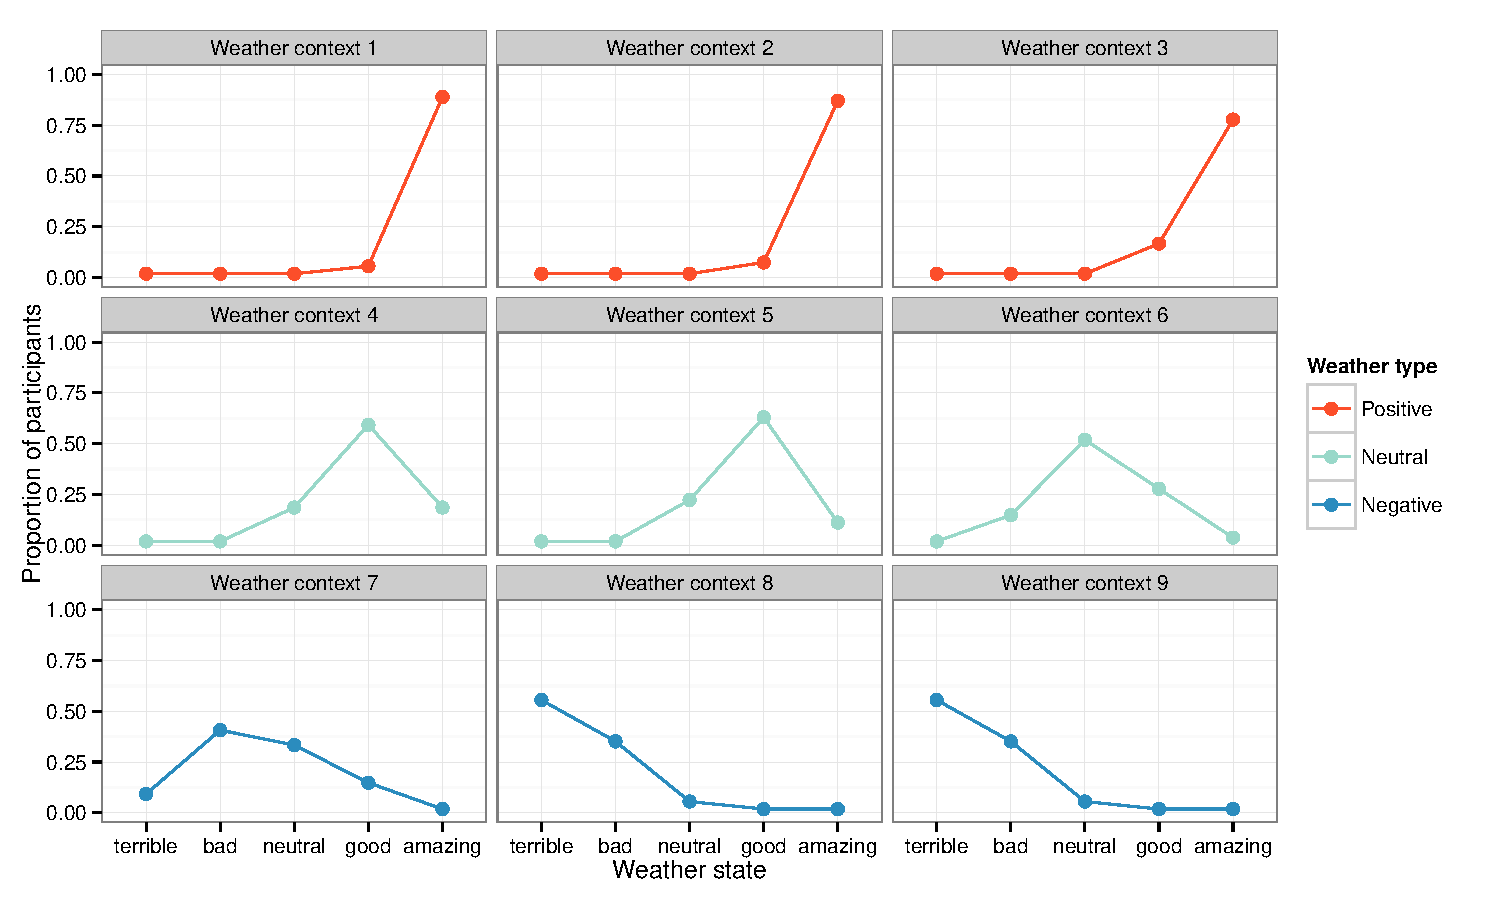
\includegraphics{priors.pdf}}
\end{figure}

\begin{figure}[t]
\scalebox{0.6}{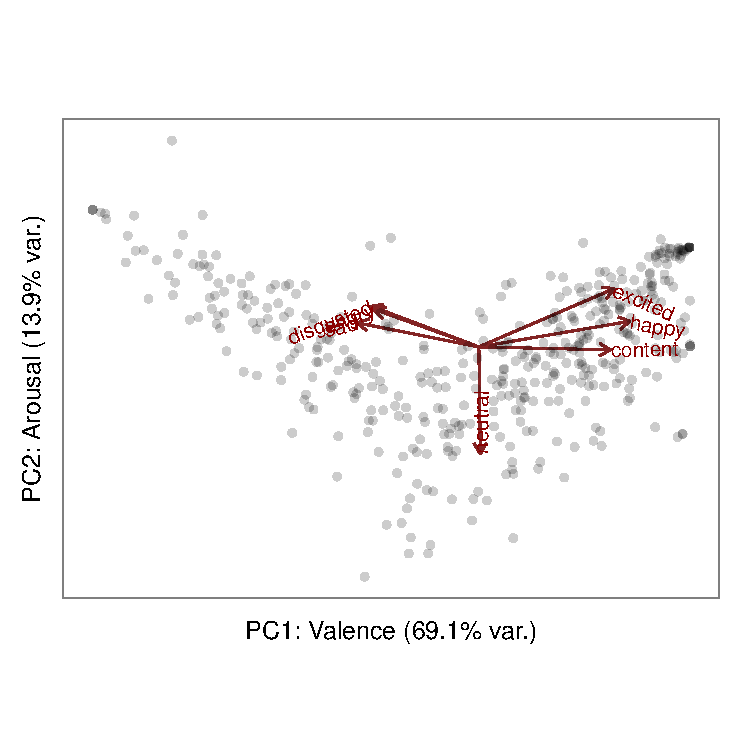
\includegraphics{biplot.pdf}}
\end{figure}

\begin{figure}[t]
\scalebox{0.6}{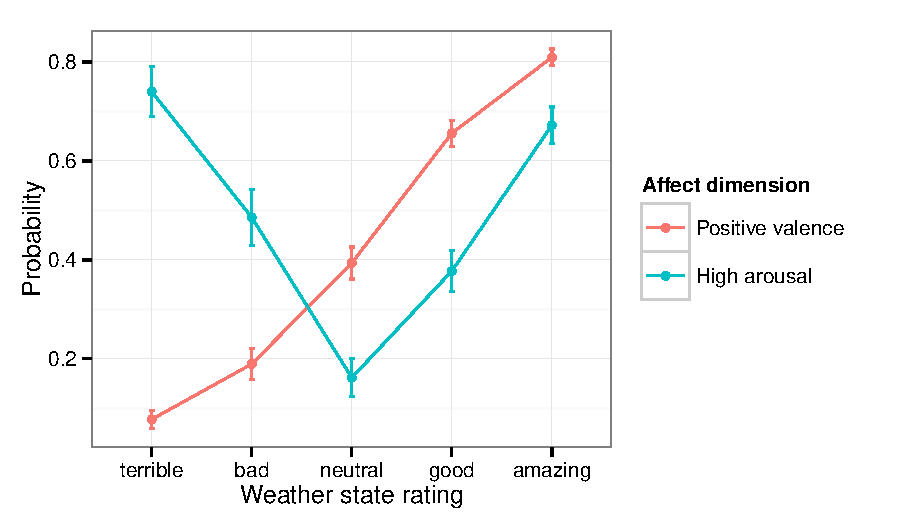
\includegraphics{affect-prior.pdf}}
\end{figure}
For each of the nine weather contexts, we obtained the number of participants who gave each of the weather state ratings and performed add-one Laplace smoothing on the counts. This allowed us to compute a smoothed prior distribution over weather states given each context (see Figure XX). 
%
To examine participants' ratings of the affects associated with each context, we first performed Principal Component Analysis (PCA) on the seven emotion category ratings. This allowed us to compress the ratings onto a lower-dimensional space and also reveal the main affective dimensions that are important in this domain. We found that the first two principal components accounted for $69.14\%$ and $13.86\%$ of the variance in the data (see Figure XX). In addition, they correspond roughly to the dimensions of emotional valence (positive or negative) and emotional arousal (high or low), respectively, which are consistent with theories of emotion in affective science (cite). In order to examine the probabilities of Ann feeling positive or negative affect and high or low arousal given different weather states, we performed a series of transformations to convert the PCA scores into probabilities. We first normalized the scores in each dimension to have zero mean and unit variance. Treating these normalized scores as quantiles of a standard normal distribution, we used the cumulative distribution function to convert the normalized scores into values between $0$ and $1$. (TODO: something about how this is not a perfect transformation but does approximately the right thing) Figure XX shows the probability of positive valence and high arousal given each weather state.

%\begin{figure}
%\begin{minipage}[b]{.5\textwidth}
%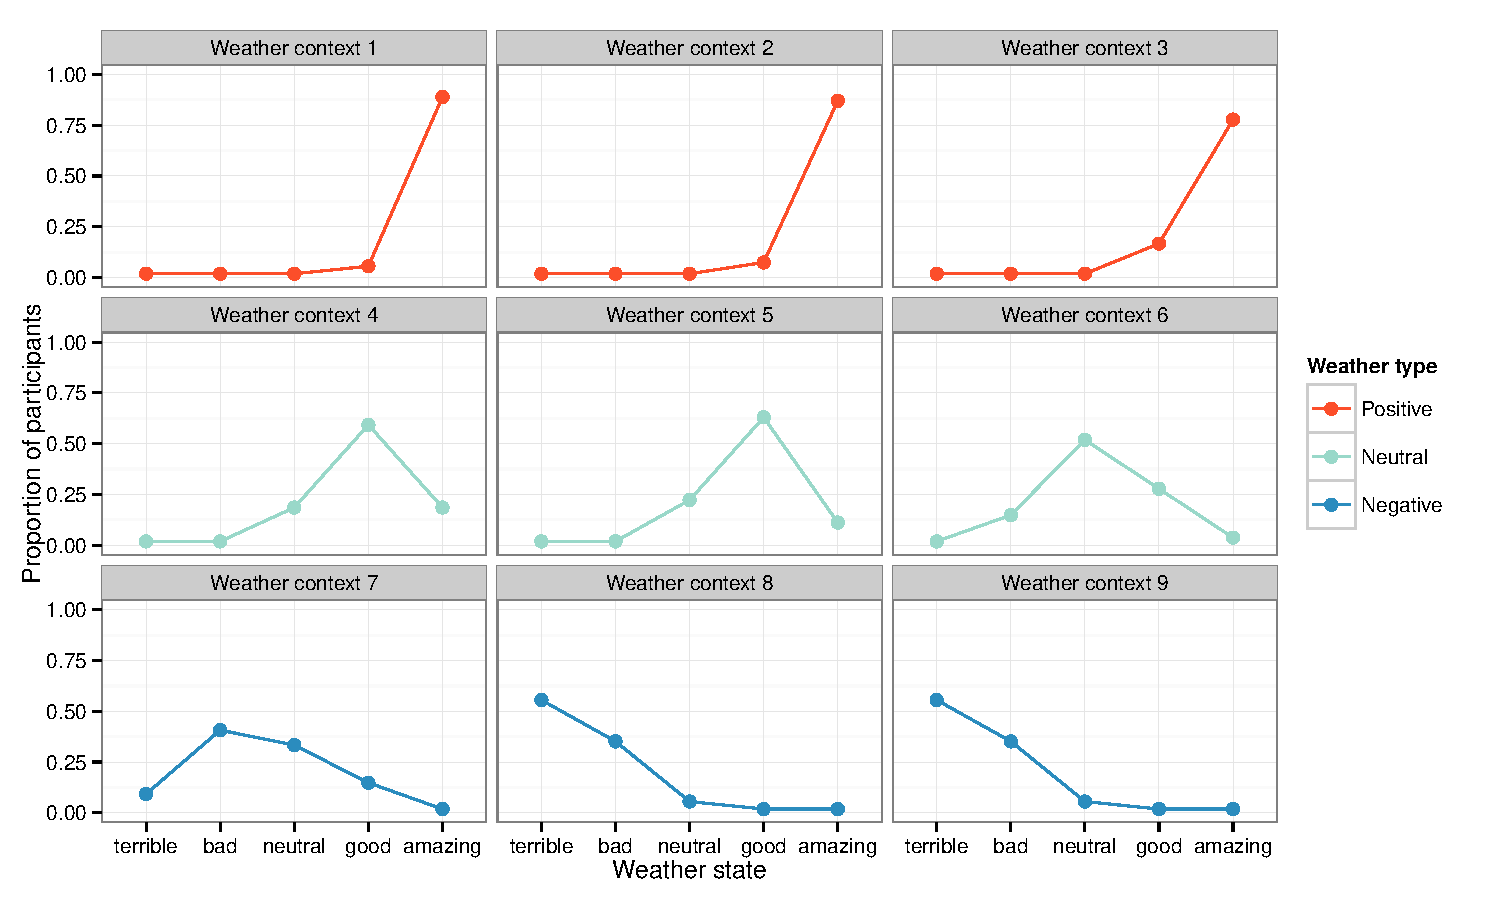
\includegraphics[width=5cm, height=3.7cm]{priors.pdf}
%\end{minipage}
%\begin{minipage}[b]{.4\textwidth}
%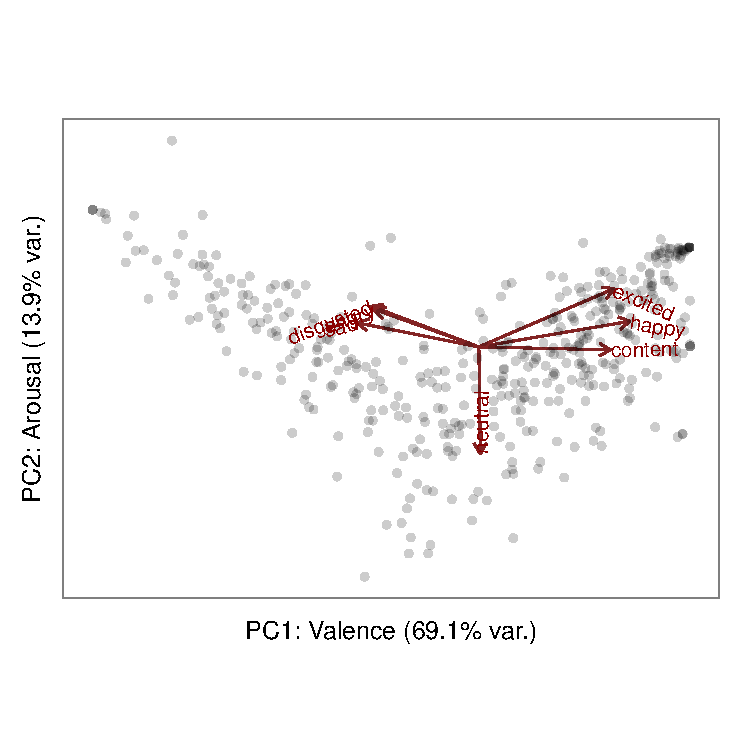
\includegraphics[width=5cm, height=5cm]{biplot.pdf}
%\end{minipage}
%
%\end{figure}

\subsection{Experiment 2: Irony understanding}
\subsubsection{Materials and methods}
We used the same nine weather images from Experiment 1. $59$ native English speakers with IP addresses in the United States were recruited on Amazon's Mechanical Turk. Each participant saw all nine images in random order. In each trial, participants were told that Ann (characters' names were randomized) and her friend look out the window together and sees the view depicted by the image. Ann says, ``The weather is \underline{\hspace{1cm}}!" where the adjective is randomly selected at each trial from the following set: ``terrible," ``bad," ``ok," ``good," and ``amazing." Participants first rated how likely it is that Ann's statement is ironic using a slider with end points labeled ``Definitely NOT ironic" and ``Definitely ironic." They then indicated how Ann would actually rate the weather using a labeled 5-point Likert scale, ranging from \emph{terrible}, \emph{bad}, \emph{neutral}, \emph{good}, to \emph{amazing}. Finally, participants used sliders to rate how likely it is that Ann feels each of the seven emotions about the weather. A link to the experiment is here:

\subsubsection{Results}
We first examined participants' irony ratings for each of the weather context and utterance pairs. We coded ``terrible" and ``bad" as \emph{negative} utterances, ``ok" as a \emph{neutral} utterance, and ``good" and ``amazing" as \emph{positive} utterances. We also coded each image as \emph{positive, neutral}, or \emph{negative} based on the modal weather state rating from Experiment 1 (e.g. $w_1$ is \emph{positive}, $w_6$ is \emph{neutral}, and $w7$ is \emph{negative}). We found a basic irony effect, where utterances whose polarities are inconsistent with the polarity of the weather context (e.g. using ``terrible" to describe $w_1$) are rated as significantly more ironic than utterances whose polarities are consistent with the weather context (e.g. using ``good" or ``amazing" to describe $w_1$) (STATS) (Figure XX?). Furthermore, a linear regression model with the polarity of the utterance, the polarity of the weather context, and their interaction as predictors of irony ratings produced an adjusted R-squared of 0.91, capturing most of the variance in the data. 

\begin{figure}[t]
\scalebox{0.45}{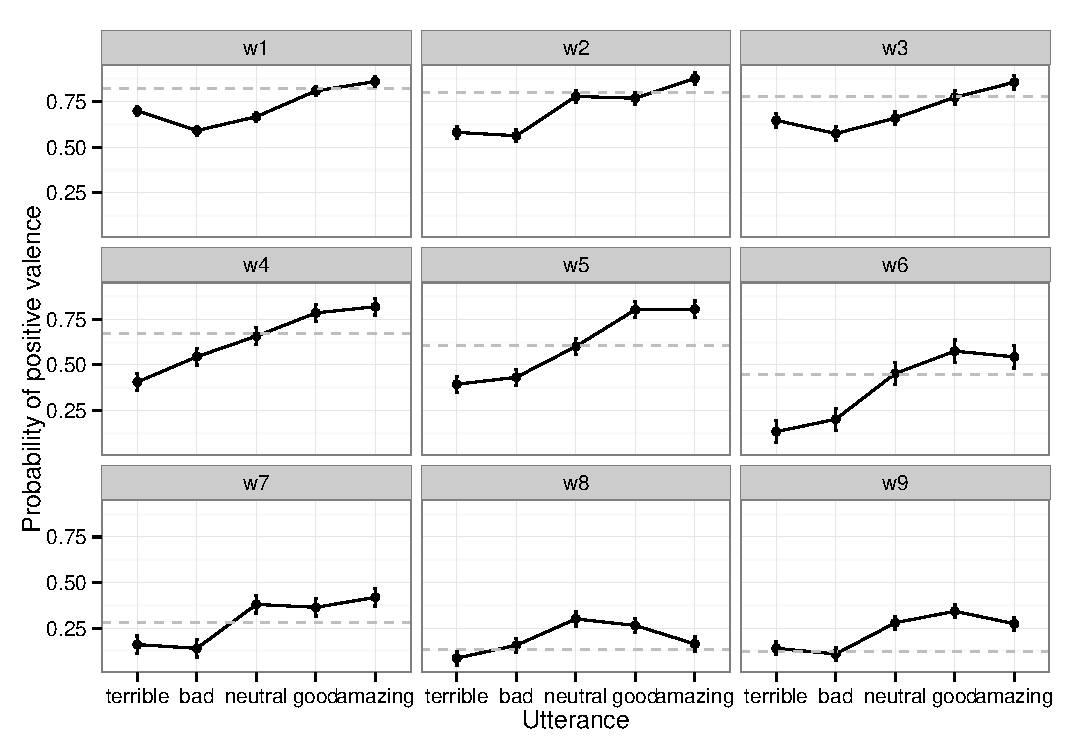
\includegraphics{valence.pdf}}
\end{figure}

\begin{figure}[t]
\scalebox{0.45}{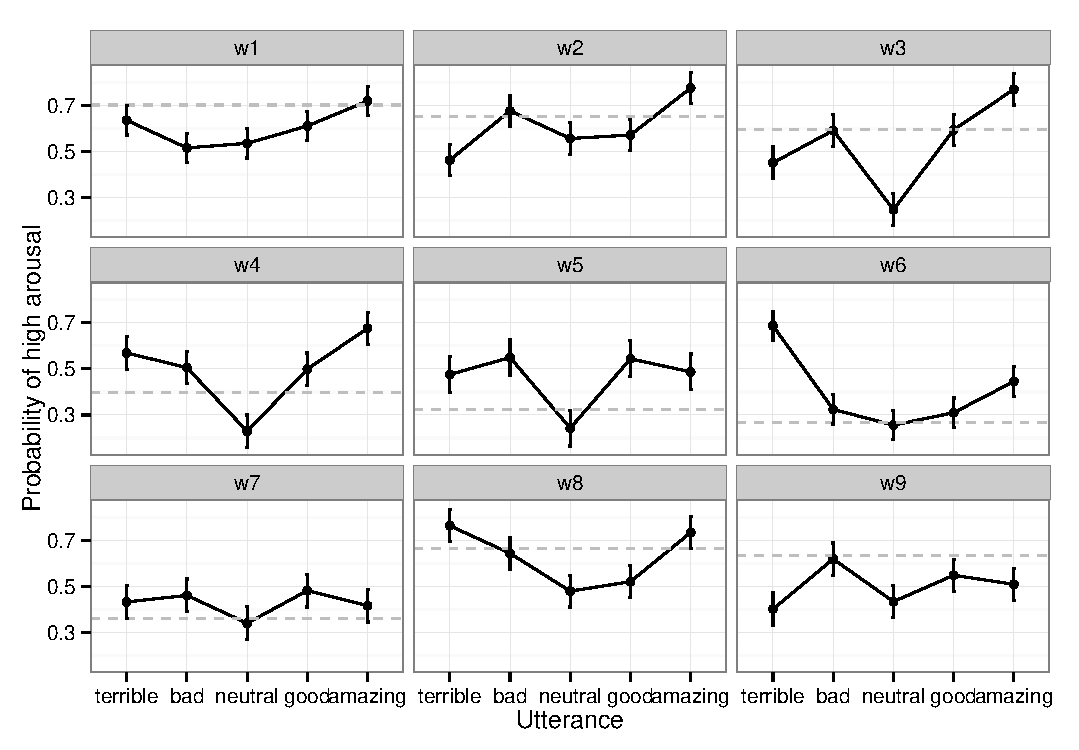
\includegraphics{arousal.pdf}}
\end{figure}

We then examined participants' ratings of the weather context given an utterance. For each of the $45$ weather context (9) $\times$ utterance (5) pairs, we obtained the number of participants who gave each of the five weather ratings. After performing add-one Laplace smoothing on the counts, we computed a smoothed distribution over weather states given each context and utterance (Figure XX?). We call this distribution the \emph{interpreted meaning} of an utterance in context. We found that participants often rated the speaker (e.g. Ann) as judging the actual weather state to be different from what she described in her utterance, suggesting that participants interpreted these utterances non-literally. To further examine the relationship between literal meaning, interpreted meaning, and judgements of irony, we computed the Kullback-Leibler divergence between the literal interpretation of the utterance and the distribution over weather states given the context and utterance. We found that adding the KL divergence measure to the linear regression model captured significantly more variance in the irony ratings, with an R-squared of 0.93 (more STATS). This suggests that even beyond inconsistencies in polarity between utterance and context, people are sensitive to the fine-grained differences between literal and interpreted meanings in their judgements of irony.

Finally, we examined the emotions expressed by utterances in context. We used the loadings from the PCA on emotion ratings from Experiment 1 to predict the projected values of emotion ratings in Experiment 2 and performed the same transformations on the scores to convert them into values between $0$ and $1$. Figure XX shows the average probability of positive valence given a weather context and an utterance. The dotted gray lines are the average probabilities of positive valence associated with each weather context without any linguistic input, taken from Experiment 1. We see that for the \emph{positive} weather contexts ($w_1, w_2, w_3$), the speaker is interpreted as more likely expressing positive valence given the extremely negative utterance ``terrible" than given the less negative utterance ``bad." On the other hand, for the \emph{negative} weather contexts ($w_7, w_8, w_9$), the speaker is interpreted as less likely expressing positive valence given the extremely positive utterance ``amazing than the less positive utterance ``good" (STATS). This suggests that extreme utterances that are inconsistent with the valence of the context are more likely to express an opposite affect than its literal meaning (MAKE THIS CLEARER).

Figure XX shows the average probability of high arousal given a weather context and an utterance. The dotted gray lines are the average probabilities of high arousal associated with each weather context without any linguistic input, taken from Experiment 1. We see that regardless of the weather context, more extreme utterances are more likely to express high arousal (MAKE THIS CLEARER). (Generally, just say that the utterance shifts interpreted valence and arousal away from the baseline). 

\section{Computational Model}
Our behavioral experiments confirmed that people's judgments of irony are highly sensitive to their prior knowledge of the world. We also showed that two affective dimensions---valence and arousal---may be especially important for irony. Here we describe an extension to the basic Rational Speech Act (RSA) model that incorporates these elements to produce interpretations of ironic utterances. 

In RSA models, a speaker chooses an utterance that most effectively communicates her intended meaning to a literal listener; a pragmatic listener then reasons about the speaker to infer a pragmatically enriched meaning given the utterance \cite{frank2012predicting, goodman2013knowledge}. To model nonliteral language understanding, \cite{kao2014nonliteral} extended the basic RSA model to incorporate an affective dimension of meaning and multiple communicative goals, opening up the possibility for a speaker to produce an utterance that is literally false but satisfies her goal to convey affect. The extended model was able to produce appropriate interpretations of hyperbole as well as its affective subtext. However, since the model only considered a fairly impoverished affect goal (communicating presence or absence of negative affect), it could not take into account cases where a negative utterance is used to communicate positive affect (and vice versa), which is critical in ironic uses (e.g. saying ``Life is so hard!" when sipping iced lemonade on a sunny beach). 

Drawing from our analysis of affect in Experiment 1 and 2, we extend the interpreted meaning of an utterance to have the following dimensions: the weather state $s$, where $s \in \{$\emph{terrible, bad, neutral, good, amazing}$\}$; the speaker's emotional valence $v$ towards the weather state, where $v \in \{$\emph{positive, negative}$\}$, and her emotional arousal $a$ towards the weather state, where $a \in \{$\emph{high, low}$\}$. We consider the interpreted meanings of utterances $u$ in the following set: $\{$``terrible," ``bad," ``ok," ``good," ``amazing"$\}$. 

We begin with a literal listener $L_0$, who interprets all utterances literally. For example, the literal listener will interpret the utterance ``The weather is terrible" to mean that the weather state $s=$\emph{terrible}, and that the speaker has the corresponding valence and arousal towards the weather. Formally, if $u$ is the uttered adjective:
\[ L_0(s, v, a|u) = \left\{ 
  \begin{array}{l l}
    P(v, a | s) & \quad \text{if $s$ = $u$}\\
    0 & \quad \text{otherwise}
  \end{array} \right.\]
where $P(v, a | s)$ is the prior probability that a speaker would feel valence $v$ and arousal $a$ towards the weather state $s$.

We assume that the speaker's goal $g$ is to communicate  along any (or multiple) of the three dimensions of meaning, which results in $2^3 - 1 = 7$ possible goals (the speaker cannot communicate along none of the dimensions). For example, the speaker may want to communicate only the weather state $s$, or only her valence about $s$, or both.
A goal is thus a projection from the full meaning space to the subset of interest to the speaker. Following the Rational Speech Act model, we define the speaker's utility as the negative surprisal of the true state under the listener's distribution, given an utterance. However, here we consider only the surprisal along the goal dimension(s). 
To do so we project along the goal dimension(s), which leads to the following utility function for speaker $S_1$:
\begin{equation}
U(u | s, v, a, g) = \log \sum_{s', v', a'} \delta_{g(s, v, a)=g(s', v', a')} L_0(s, v, a |u)
\end{equation}
Given this utility function, the speaker chooses an utterance according to a softmax decision rule that describes an approximately rational planner \cite{sutton1998reinforcement}:
\begin{equation}
S_1(u | s, v, a, g) \propto e^{\lambda U(u | s, v, a, g)},
\end{equation}
where $\lambda$ is an optimality parameter. 
%
Imagine that $S_1$ has the goal to convey her emotional arousal $a$ about John. Based on $S_1$'s understanding of $L_0$'s prior knowledge, she knows that if she produces the utterance ``The weather is terrible," $L_0$ will believe that the weather is terrible and that the speaker is likely to feel high arousal about it. Since $S_1$'s goal is satisfied if the listener believes that she feels high arousal towards the weather state, $S_1$ is motivated to produce such an utterance. 

A pragmatic listener $L_1$ takes into account prior knowledge and his internal model of the speaker to determine the intended meaning. Because the pragmatic listener is uncertain about which goal the speaker has, $L_1$ will marginalize over the possible speaker goals under consideration:
$$
L_1 (s, v, a | u) \propto P(s) P(v, a | s) \sum_{g}{P (g) S_1 (u|s, v, a, g)}
$$
%While speaker and listener could continue to reason about each other recursively, resulting in $L_n$, we restrict ourselves to $L_1$ for present purposes. Past work has shown that this first level of pragmatic reasoning is often a good model of human comprehension.
If $L_1$ thinks it is likely that speaker $S_1$'s goal is to convey high arousal but believes (e.g. based on visual evidence) that it is \emph{a priori} very likely that the actual weather state is \emph{amazing} instead of \emph{terrible}, he will determine that $S_1$ is using her utterance ``The weather is terrible!" ironically, and that the weather is, in fact, \emph{amazing}, and the speaker feels positive valence and high arousal about it. Common knowledge of a domain (e.g. the weather and associated affects) and reasoning about communicative goals thus allows the pragmatic listener to infer the appropriate nonliteral and affective meanings from an ironic utterance.

\section{Model Evaluation}
In this section, we evaluate the model's performance using results from our behavioral experiments. To produce an interpretation of an utterance in context, the model requires the following input values: (1) the prior probability of a weather state $s$ for a given weather context, $P(s)$ (2) the joint probability of positive/negative valence given a weather state, $P(v, a | s)$ (3) the prior probability of a particular goal $P(g)$ (4) the speaker optimality parameter $\lambda$. We derived the values for (1) and (2) from Experiment 1 and fit (3) and (4) to the data from Experiment 2 (TODO: add actual fit values in a clear manner: $\lambda=1$, p(state goal) = 0.2, p(valence goal) = 0.3, p(arousal goal)=0.4).

The model produced an interpretation for each of the $45$ utterance $\times$ weather context pairs. Each interpretation is a joint posterior distribution $P(s, v, a | u)$. We first examine the model's performance on recovering the actual weather state $P(s | u)$ by marginalizing over $v$ and $a$. Figure XX shows participants' and the model's interpretation of the actual weather state given an utterance and a weather context. We see that the model predictions closely match humans' interpretations, with a correlation of $0.86$ (show scatter plot?). Next, we examine the model's performance on recovering the speaker's valence by marginalizing over $s$ and $a$. The model's prediction for emotional valence match humans' extremely closely, with a correlation of $0.96$. Finally, we examine the model's performance on recovering the speaker's emotional arousal by marginalizing over $s$ and $v$. The model's prediction for emotional arousal match humans' with a correlation of $0.66$ (TODO: add split half; figures???). This suggests that the model is able to incorporate background knowledge and reasoning about multiple affective goals to produce the appropriate ironic interpretations as well as the associated affects. 

\begin{figure}[t]
\scalebox{0.5}{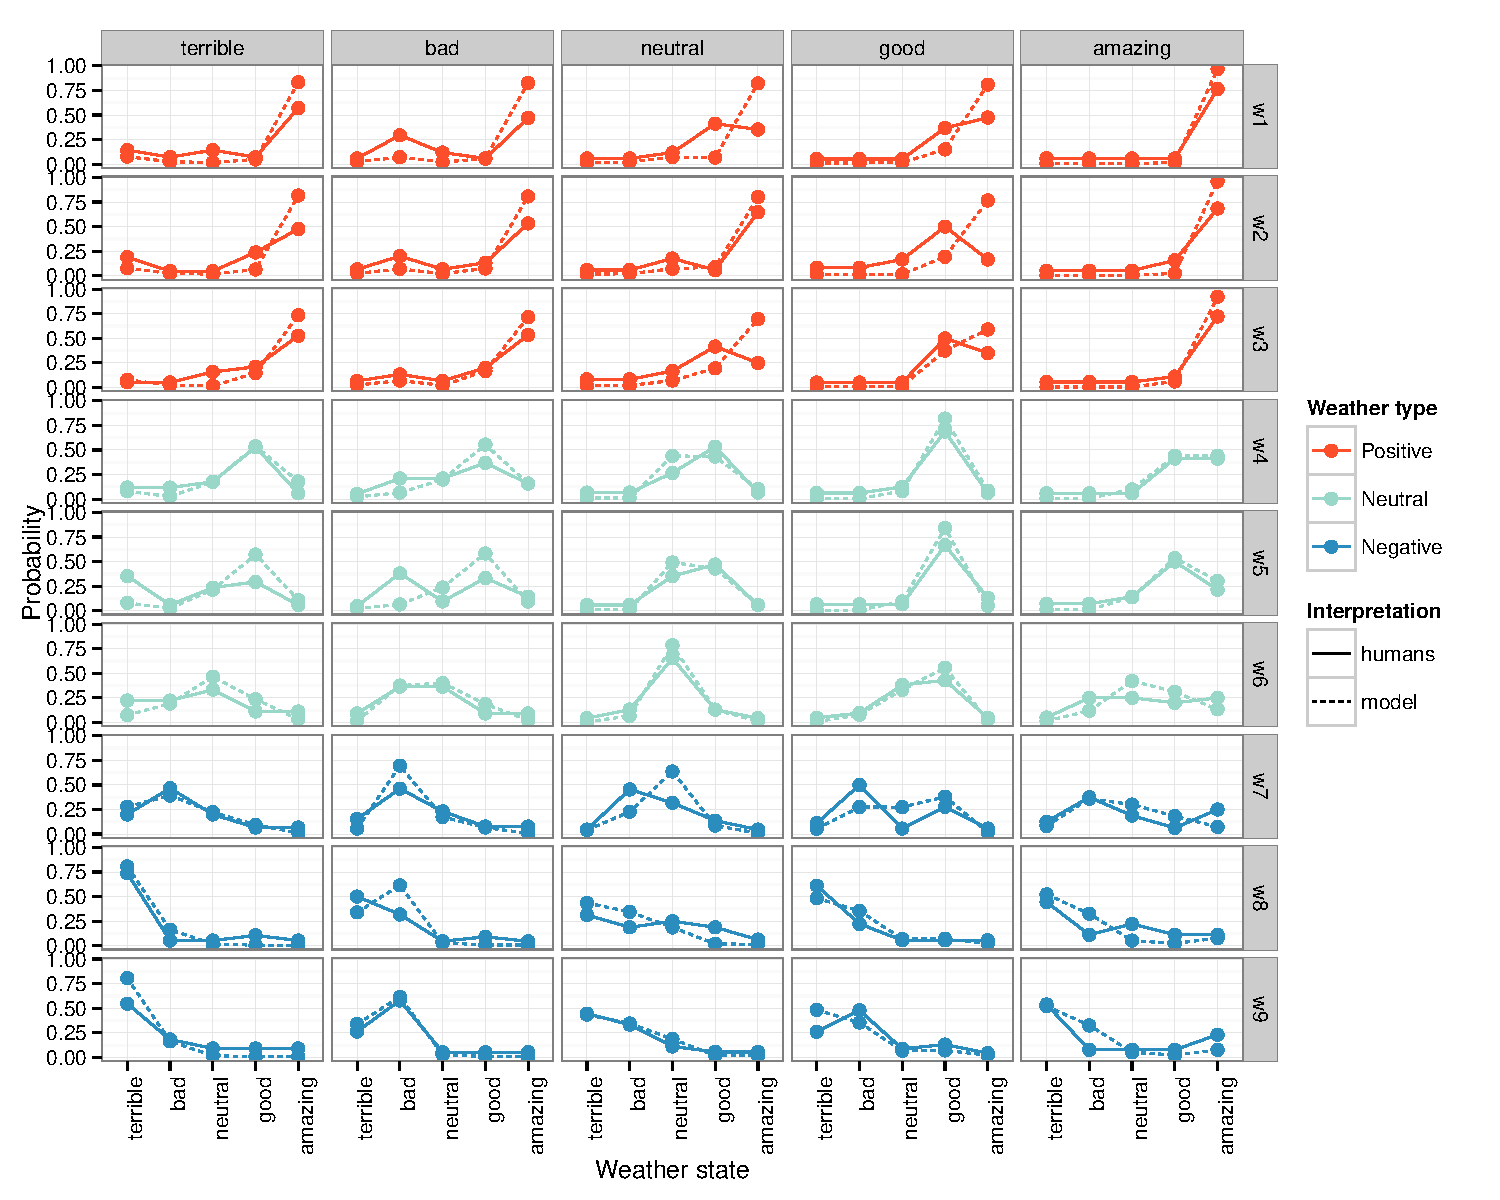
\includegraphics{model-state.pdf}}
\end{figure}

\section{Discussion}

With our behavioral experiments, we presented results showing the fine-grained effects of background knowledge on people's interpretations of ironic utterances, and identified the main affective dimensions that are conveyed by irony. In addition, we presented a computational model that predicts peoples' interpretations of ironic utterances using general communicative principles. In effect, the model is able to tell when an utterance is meant to be literal or ironic, and when meant to be ironic, what types of affect the speaker intends to convey. By reasoning about the speaker's communicative goals, the model goes beyond the literal meaning of an utterance to infer the actual state of the world. In addition, it recovers important aspects of the speaker's affect about the situation and captures the social and affective uses of irony. Together, these results suggest that basic principles of communication---background knowledge and reasoning about informativeness with respect to the speaker's communicative goals---may be an important driver of irony understanding.

It is important to note that the model we present here is only minimally different from the hyperbole model described earlier in the paper \cite{kao2014nonliteral}. In fact, the only difference is that instead of considering a single affect dimension (negative valence), this extended model takes seriously the circumplex model of affect (cite), which identifies valence and arousal as two main dimensions underlying the slew of emotions people experience. The similarities between these two models suggests that hyperbole and irony may be understood using similar principles of communication. A deeper point we wish to make with this work is that communication in general, and nonliteral language understanding in particular, relies on reasoning about the speaker's communicative goals during interpretation. Furthermore, these goals are often social or affective in nature, and speakers are adept at harnessing shared background knowledge with the listener to convey rich affective meanings without explicitly stating them. 

Our experimental paradigm and modeling framework lends itself well to a more detailed and precise account of irony understanding. For example, what are the range of social and affective meanings involved in irony understanding? We identified emotional valence and arousal in these experiments, but there may be others ....(attitudes? opinions? affect? social closeness?)
(TODO: finish) What are the social functions of irony? Irony is often used to signal social closeness with the listener, presumably because it expresses the speaker's assumption that she and the listener share a great deal of common ground (cite). Given an ambiguous utterance that could be interpreted either literally or ironically, if a speaker supplements the utterance with prosodic cues to signal that it is meant ironically, will listeners judge the speaker as being closer to them? Can our model more directly  test the predictions of the echoic mention and pretense theories of irony and help distinguish between them? Given the prevalence of irony in everyday language, we believe it would be \emph{amazing} (literally) to address these questions in future research and understand irony's mysterious ability to be interpreted as the opposite of what it is.

\bibliographystyle{apacite}

\setlength{\bibleftmargin}{.125in}
\setlength{\bibindent}{-\bibleftmargin}

\bibliography{irony}


\end{document}
